%%%%%%%%%%%%%%%%%%%%%%%%%%%%%%%%%%%%%%%%%
% Wenneker Assignment
% LaTeX Template
% Version 2.0 (12/1/2019)
%
% This template originates from:
% http://www.LaTeXTemplates.com
%
% Authors:
% Vel (vel@LaTeXTemplates.com)
% Frits Wenneker
%
% License:
% CC BY-NC-SA 3.0 (http://creativecommons.org/licenses/by-nc-sa/3.0/)
% 
%%%%%%%%%%%%%%%%%%%%%%%%%%%%%%%%%%%%%%%%%

%----------------------------------------------------------------------------------------
%	PACKAGES AND OTHER DOCUMENT CONFIGURATIONS
%----------------------------------------------------------------------------------------

\documentclass[12pt]{scrartcl} % Font size

%%%%%%%%%%%%%%%%%%%%%%%%%%%%%%%%%%%%%%%%%
% Wenneker Assignment
% Structure Specification File
% Version 2.0 (12/1/2019)
%
% This template originates from:
% http://www.LaTeXTemplates.com
%
% Authors:
% Vel (vel@LaTeXTemplates.com)
% Frits Wenneker
%
% License:
% CC BY-NC-SA 3.0 (http://creativecommons.org/licenses/by-nc-sa/3.0/)
% 
%%%%%%%%%%%%%%%%%%%%%%%%%%%%%%%%%%%%%%%%%

%----------------------------------------------------------------------------------------
%	PACKAGES AND OTHER DOCUMENT CONFIGURATIONS
%----------------------------------------------------------------------------------------

\usepackage{amsmath, amsfonts, amsthm} % Math packages

\usepackage{listings} % Code listings, with syntax highlighting

\usepackage[english]{babel} % English language hyphenation

\usepackage{graphicx} % Required for inserting images
\graphicspath{{Figures/}{./}} % Specifies where to look for included images (trailing slash required)

\usepackage{booktabs} % Required for better horizontal rules in tables

\numberwithin{equation}{section} % Number equations within sections (i.e. 1.1, 1.2, 2.1, 2.2 instead of 1, 2, 3, 4)
\numberwithin{figure}{section} % Number figures within sections (i.e. 1.1, 1.2, 2.1, 2.2 instead of 1, 2, 3, 4)
\numberwithin{table}{section} % Number tables within sections (i.e. 1.1, 1.2, 2.1, 2.2 instead of 1, 2, 3, 4)

\setlength\parindent{0pt} % Removes all indentation from paragraphs

\usepackage{enumitem} % Required for list customisation
\setlist{noitemsep} % No spacing between list items

%----------------------------------------------------------------------------------------
%	DOCUMENT MARGINS
%----------------------------------------------------------------------------------------

\usepackage{geometry} % Required for adjusting page dimensions and margins

\geometry{
	paper=a4paper, % Paper size, change to letterpaper for US letter size
	top=2cm, % Top margin
	bottom=2cm, % Bottom margin
	left=2cm, % Left margin
	right=2cm, % Right margin
	headheight=0.75cm, % Header height
	footskip=1.5cm, % Space from the bottom margin to the baseline of the footer
	headsep=0.75cm, % Space from the top margin to the baseline of the header
	%showframe, % Uncomment to show how the type block is set on the page
}

%----------------------------------------------------------------------------------------
%	FONTS
%----------------------------------------------------------------------------------------

\usepackage[utf8]{inputenc} % Required for inputting international characters
\usepackage[T1]{fontenc} % Use 8-bit encoding

\usepackage{fourier} % Use the Adobe Utopia font for the document

%----------------------------------------------------------------------------------------
%	SECTION TITLES
%----------------------------------------------------------------------------------------

\usepackage{sectsty} % Allows customising section commands

\sectionfont{\vspace{6pt}\centering\normalfont\scshape} % \section{} styling
\subsectionfont{\normalfont\bfseries} % \subsection{} styling
\subsubsectionfont{\normalfont\itshape} % \subsubsection{} styling
\paragraphfont{\normalfont\scshape} % \paragraph{} styling

%----------------------------------------------------------------------------------------
%	HEADERS AND FOOTERS
%----------------------------------------------------------------------------------------

\usepackage{scrlayer-scrpage} % Required for customising headers and footers

\ohead*{} % Right header
\ihead*{} % Left header
\chead*{} % Centre header

\ofoot*{} % Right footer
\ifoot*{} % Left footer
\cfoot*{\pagemark} % Centre footer
 % Include the file specifying the document structure and custom commands

%----------------------------------------------------------------------------------------
%	TITLE SECTION
%----------------------------------------------------------------------------------------
\usepackage{float}
\title{	
	Homework 5
}
\usepackage{float}
\usepackage{xcolor}
\lstset{
    columns=fixed,       
    numbers=left,                                        % 在左侧显示行号
    frame=none,                                          % 不显示背景边框
    backgroundcolor=\color[RGB]{245,245,244},            % 设定背景颜色
    keywordstyle=\color[RGB]{40,40,255},                 % 设定关键字颜色
    numberstyle=\footnotesize\color{darkgray},           % 设定行号格式
    commentstyle=\it\color[RGB]{0,96,96},                % 设置代码注释的格式
    stringstyle=\rmfamily\slshape\color[RGB]{128,0,0},   % 设置字符串格式
    showstringspaces=false,                              % 不显示字符串中的空格
    language=c++,                                        % 设置语言
}
\author{Yuan Jiahao 2019010070} % Your name

\date{\normalsize\today} % Today's date (\today) or a custom date

\begin{document}

\maketitle % Print the title

%----------------------------------------------------------------------------------------
%	FIGURE EXAMPLE
%----------------------------------------------------------------------------------------

\section{Todo}
 (1) Run the given SUMMA MPI code for distributed GEMM. Try to change the number of
processes (1, 2, 4 should be enough for this homework) to parallelize them, verify the correctness
of the results, test performance, and write them in the report;

(2) Try to find the difference between MPI and OpenMP programming model, and recall
the difference between process and thread.
\section{Hardware Environment of the Machine }
The machine's CPU is Intel Core i3-10100F ,3.2GHz with 4 cores and 8 threads.The memory is 16GB,the GPU is two NVIDIA GTX-1650 crossfire,and the system is Ubuntu 20.04.

All the following codes are complied in O3 optimization and nvcc option is -gencode $=$ arch $=$ compute\_61, code$=$compute\_61.
\section{Analysis}
Since the node num should can be sqrt,so number 2 is an illegal input,thus I guess 2 is misplaced inside the requirement 1,2,4.And what we are required to do is just measure one process and four processes's performance.But in case I misunderstood it,the performance of 1 process,4 processes and 16 processes will be shown below.

\subsection{What is SUMMA}
Summa divide matrix A,B and C into small blocks,and calculate the multiplication of each block.Finally gather the result and merge them.Thus we can split a great matrix multiplication problem into small problems,and solve them in parallel in different nodes.
\section{Result}
\subsection{Running time}
\begin{figure}[H]
    \centering
    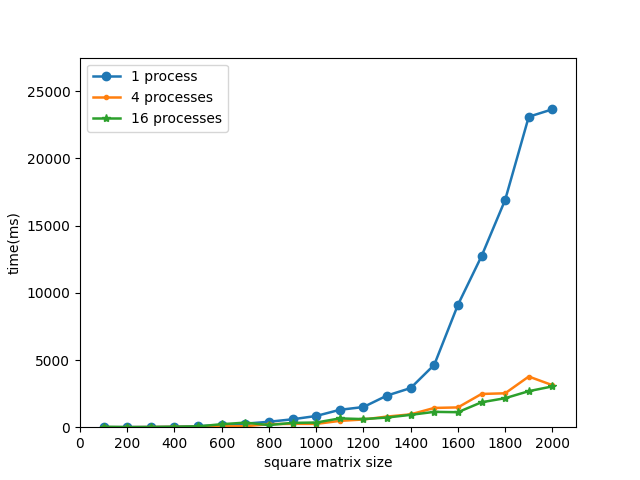
\includegraphics[width=0.85\textwidth]{4.png}
    \caption{running time}
\end{figure}
Just as the running time before,there always will be a very slow method and makes others hard to compare.

So,it might be a better choice to have a GFLOPS chart:
\begin{figure}[H]
    \centering
    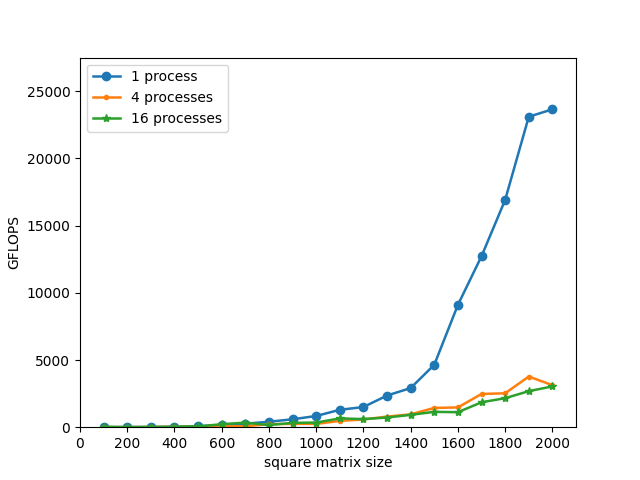
\includegraphics[width=0.85\textwidth]{3.png}
    \caption{GFLOPS performance}
\end{figure}
As we can see,as the number of processes increase from one to four,the GFLOPS increases greatly,but when the number of processes increase to 16,the performance doesn't have a obvious improvement,which might due to our CPU only have 4 cores and 8 threads,too much processes doesn't make any sense.

Also,when the number of processes is fixed,we still see a great fluctuation,so the performance of our CPU program is not very stable.

\subsection{The difference between MPI and OpenMP  programming model}
When we write OpenMP program,we don't care the data exchange between threads,since they share the same memory space.Meanwhile,we don't care how many threads are created or destroyed,since the cost of thread creation and destruction is not so much.

However,when we write MPI program,we need to explicitly transfer the data between processes,and we create few processes before the start of program,rather than creating lots of processes during the program running.

The result is that MPI program can be distributed across different nodes,and OpenMp merely can be distributed across different cores in one node.

Thus,the programming model will be very different when we choose MPI or OpenMP.
\subsection{The difference between processes and threads}
Processes and threads are all developed to solve parallel problems.And in some cases both of them can have their own registers,context etc.However,processes can't share memory space,and they must define their socket to communicate.When it comes to threads,only if they belong to the same process,they can share memory space.

Thus, the creation,switch cost of threads are much smaller than processes,it's very common a process has a great deal of threads.

Finally,the reliability is different between these two staff.When a thread crash,the whole process will crash too.But process will not affect another process.
\end{document}